Prescribing to the school of thought: ``the more data the better'', we used all of the 40,000+ human patches as training data.
Although there are some spurious patches, a majority are good, hence we choose to use all the patches (see Figure \ref{fig:Q1_3}).
It may have been beneficial to standadize the size of the training dataset, equalizing class sizes and games/movies split.
But this was not something we investigated.

We also trained a background model.
For this dataset we removed the first and last 2 seconds of movie data (fade in and fade out).

\begin{figure}[h!]
  \begin{center}
  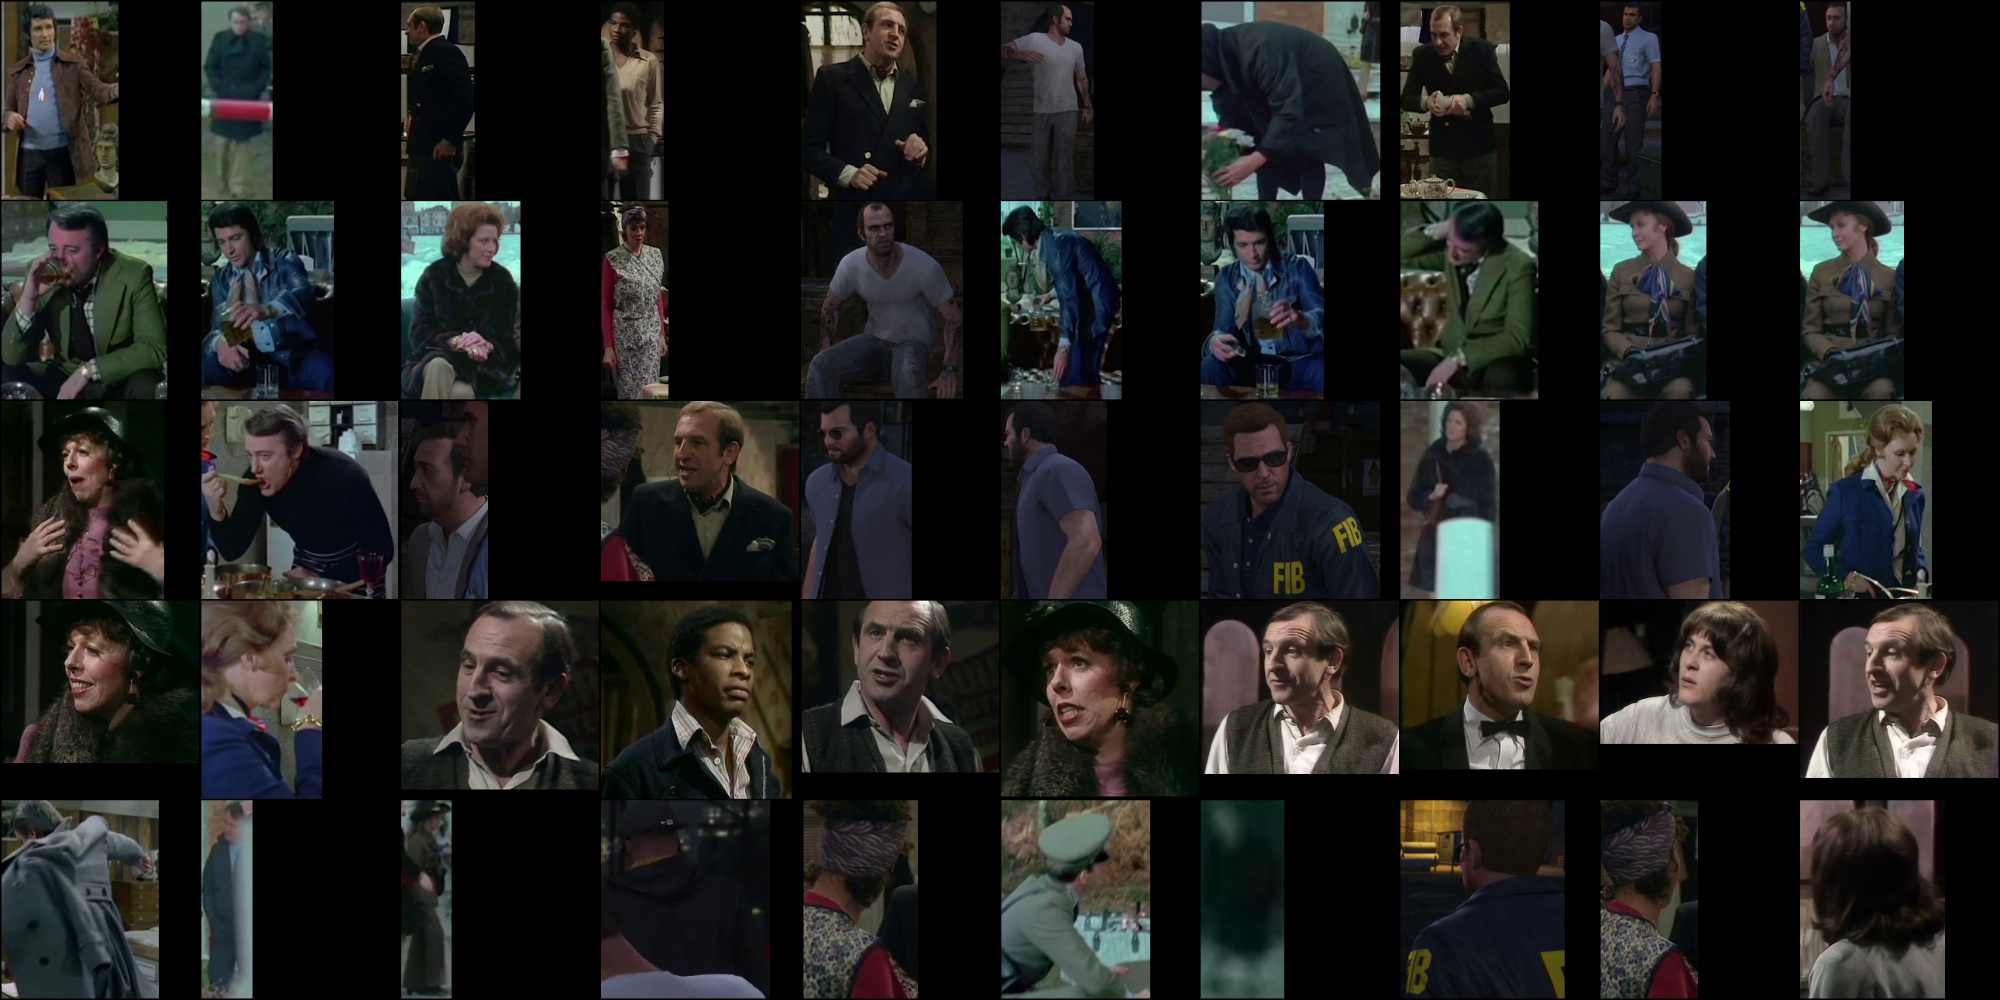
\includegraphics[scale=0.2]{Q1_3_full.jpg}
    \caption{Q1.3 sample of classified human patches. From top to bottom each row is class: full-body, sitting, half-body, head, other.}
    \label{fig:Q1_3}
  \end{center}
  \end{figure}